\section{Cluster Reconstruction}

Particles impacting the calorimeter produce localized energy depositions or ${\it clusters}$.  Cluster reconstruction starts with the identification of scintillator strips having energy above a user-defined threshold as ${\it hits}$, and grouping contiguous hits into one or more ${\it peaks}$.  The criterion for a cluster requires the spatial intersection of three peaks, one from each of the U, V, and W stereo views.  Each peak is represented geometrically as a three-dimensional line determined by the energy-weighted average of the mid-lines of each member strip.  The schematic shown in Fig.~\ref{fig:S6_0} describes this geometric matching procedure.  A more complete discussion can be found in \cite{nim:recon}.

Once the cluster is localized, the path from the cluster position to the PMT readout end is calculated for each
U,V,W peakline and the peak energies are corrected for scintillator light attenuation.  In addition the peak timing is corrected for propagation delay of the light, using the effective velocity of light determined for each scintillator from the calibration procedure.  For isolated clusters the cluster energy is then defined as the sum of the corrected energy from each of the U, V, and W peaks that define the cluster. For multiple overlapping clusters more sophisticated algorithms must be employed to correct the peak energy and timing data prior to cluster formation~\cite{nim:recon}.

\begin{figure}[hbt]
\centering
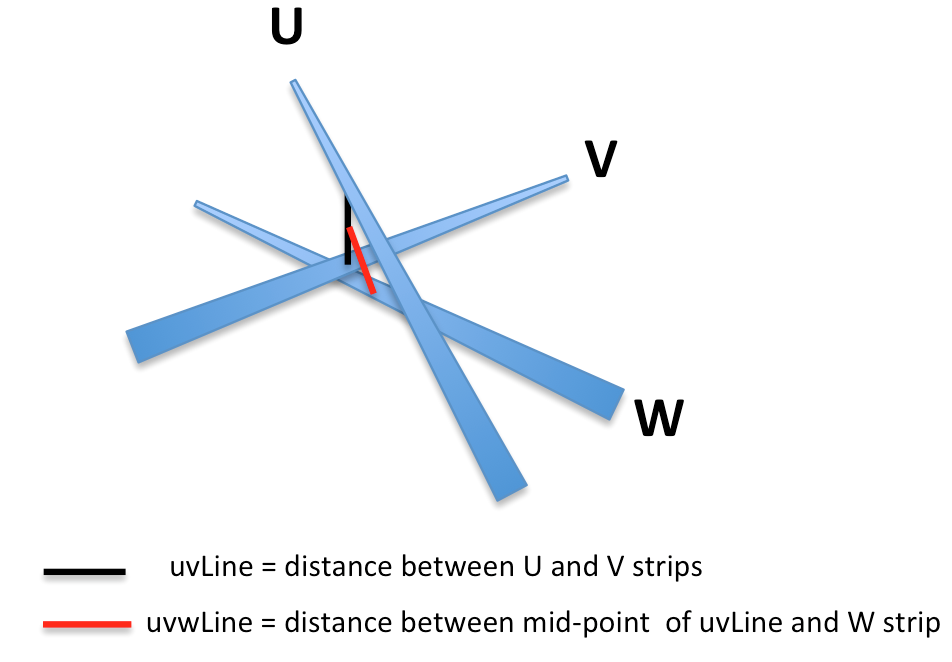
\includegraphics[width=0.95\columnwidth,keepaspectratio]{img/S6_0.png}
\caption{Schematic shows the 3D relationship of the U,V,W peaklines and the metrics used to define the cluster
  lab-frame coordinates ($x,y,z$). A cut on the length of ${\it uvwLine}$ defines the cluster, while the mid-point of ${\it uvwLine}$ defines the cluster coordinates.}
\label{fig:S6_0}
\end{figure}

Each calorimeter module of ECAL is designed to measure only the transverse ($x',y'$) position of clusters in the local frame.  In order to avoid parallax errors for tracks that are not normal to the face of the module, for PCAL the $z'$ reporting plane must be chosen to coincide with the layer of maximum energy deposition.  Similar considerations apply to barrel calorimeters~\cite{nima2018}. This effect is demonstrated in Fig.~\ref{fig:S6_1} using the CLAS12 GEANT4 simulation package GEMC~\cite{nim:sim}.  Here 2~GeV photons are generated diverging from the target position along the mid-plane and over the full polar
angle $\theta$ range of PCAL. Using a $z'$ reporting plane at the first V strip (top) clearly introduces a
$\theta$-dependent error in photon angle reconstruction, while moving this plane to the fourth V strip (bottom)
minimizes this error. For the EC module the parallax shift is compensated by the projective geometry that was
designed into the scintillators.    

\begin{figure}[hbt]
\centering
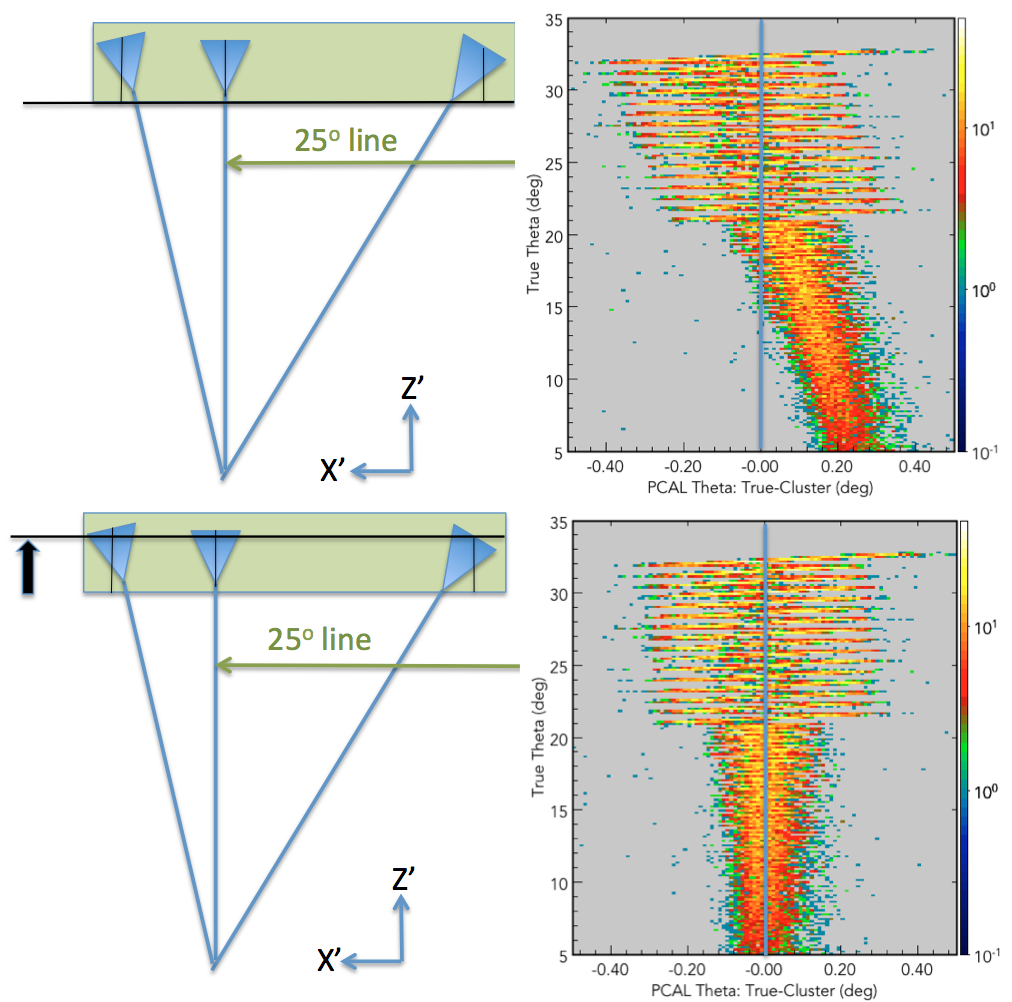
\includegraphics[width=0.95\columnwidth,keepaspectratio]{img/S6_1.png}
\caption{Left: Schematic shows how off-normal tracks with showers peaking at the rear of the calorimeter have
  a $x'$ projection at the front surface that creates parallax errors for a $z'$ reporting plane (black line) at the surface.
  Right: GEANT4 simulation of 2~GeV photons originating at the target demonstrates the error in reconstructed
  $\theta$ for $z'$ at the first V strip (top) and the fourth V strip (bottom).}
\label{fig:S6_1}
\end{figure}


